\documentclass[letterpaper]{article}
\usepackage[ascii]{inputenc}
\usepackage{amsmath}
\usepackage{amssymb,amsfonts,textcomp}
\usepackage[T1]{fontenc}
\usepackage[english]{babel}
\usepackage{color}
\usepackage{array}
\usepackage{supertabular}
\usepackage{hhline}
\usepackage{hyperref}
\usepackage[pdftex]{graphicx}
\makeatletter
\newcommand\arraybslash{\let\\\@arraycr}
\makeatother
% Page layout (geometry)
\setlength\voffset{-1in}
\setlength\hoffset{-1in}
\setlength\topmargin{1in}
\setlength\oddsidemargin{1.5in}
\setlength\textheight{9.0in}
\setlength\textwidth{5.5in}
\setlength\footskip{0.0cm}
\setlength\headheight{0cm}
\setlength\headsep{0cm}
% Footnote rule
\setlength{\skip\footins}{0.0469in}
\renewcommand\footnoterule{\vspace*{-0.0071in}\setlength\leftskip{0pt}\setlength\rightskip{0pt plus 1fil}\noindent\textcolor{black}{\rule{0.25\columnwidth}{0.0071in}}\vspace*{0.0398in}}
% Pages styles
\makeatletter
\newcommand\ps@Standard{
  \renewcommand\@oddhead{}
  \renewcommand\@evenhead{}
  \renewcommand\@oddfoot{}
  \renewcommand\@evenfoot{}
  \renewcommand\thepage{\arabic{page}}
}
\makeatother
\pagestyle{Standard}
\setlength\tabcolsep{1mm}
\renewcommand\arraystretch{1.3}
% List styles
\newcounter{saveenum}
\newcommand\liststyleWWNumi{%
\renewcommand\theenumi{\arabic{enumi}}
\renewcommand\theenumii{\arabic{enumii}}
\renewcommand\theenumiii{\arabic{enumiii}}
\renewcommand\theenumiv{\arabic{enumiv}}
\renewcommand\labelenumi{\theenumi.}
\renewcommand\labelenumii{\theenumii.}
\renewcommand\labelenumiii{\theenumiii.}
\renewcommand\labelenumiv{\theenumiv.}
}
\newcommand\liststyleWWNumii{%
\renewcommand\theenumi{\arabic{enumi}}
\renewcommand\theenumii{\arabic{enumii}}
\renewcommand\theenumiii{\arabic{enumiii}}
\renewcommand\theenumiv{\arabic{enumiv}}
\renewcommand\labelenumi{\theenumi.}
\renewcommand\labelenumii{\theenumii.}
\renewcommand\labelenumiii{\theenumiii.}
\renewcommand\labelenumiv{\theenumiv.}
}
\title{Formatting Instructions for NIPS -17-}
\author{}
\date{2023-05-23}
\begin{document}
\begin{flushleft}
\tablefirsthead{}
\tablehead{}
\tabletail{}
\tablelasttail{}
\begin{supertabular}{m{5.57126in}}
\hline
\centering\arraybslash{\selectlanguage{english} \textbf{Stroke chance prediction}}\\
\end{supertabular}
\end{flushleft}

\bigskip

{\centering\selectlanguage{english}
\textbf{Abstract}
\par}

{\selectlanguage{english}
Stroke, a leading cause of death globally, is characterized by the blockage or rupture of brain blood vessels. Metabolic
risks (e.g., high blood pressure, BMI, cholesterol) and behavioral factors (smoking, poor diet, low physical activity)
increase stroke susceptibility. This paper presents an AI model predicting stroke chances by training on a
comprehensive dataset. The model enables early detection and intervention, aiding healthcare professionals in
identifying high-risk individuals. By enhancing stroke prevention strategies, this research aims to reduce
stroke-related disabilities and deaths.}


\bigskip

{\selectlanguage{english}
\textbf{1\ \ Introduction}}


\bigskip

{\selectlanguage{english}
Stroke is a severe medical condition characterized by the interruption or rupture of blood vessels in the brain,
resulting in brain damage or potential fatality. It ranks as the second leading cause of death globally, and its
consequences can lead to long-term disabilities and diminished quality of life for survivors. The occurrence of a
stroke is influenced by a combination of metabolic risks and behavioral factors. Metabolic risks encompass high blood
pressure, elevated body-mass index (BMI), and high glucose levels.}


\bigskip

{\selectlanguage{english}
Understanding the factors that contribute to stroke risk is crucial for developing effective preventive measures and
early intervention strategies. In recent years, artificial intelligence (AI) and machine learning techniques have shown
great promise in various medical applications, including disease prediction and risk assessment. Leveraging the power
of AI, this paper presents a novel AI model designed to predict an individual's chances of experiencing a stroke based
on a comprehensive analysis of risk factors.}


\bigskip

{\selectlanguage{english}
In the following sections, we will detail the methodology employed to develop the AI model, describe the dataset
utilized for training and evaluation, present the results and analysis of the model's predictive capabilities, and
discuss the implications of this research in the context of stroke prevention and public health. Through this work, we
aim to enhance our understanding of stroke risk factors and contribute to the advancement of proactive healthcare
practices in reducing the impact of this devastating condition.}


\bigskip


\bigskip

{\selectlanguage{english}
\textbf{2.\ \ Data Description}}


\bigskip

{\selectlanguage{english}
This study utilized a comprehensive dataset containing various demographic and health-related attributes of individuals
to develop a predictive model for stroke chances. The dataset comprises the following features:}


\bigskip

\liststyleWWNumi
\begin{enumerate}
\item {\selectlanguage{english}
gender: Categorized as {\textquotedbl}Male,{\textquotedbl} {\textquotedbl}Female,{\textquotedbl} or
{\textquotedbl}Other,{\textquotedbl} this feature captures the gender of the individuals under study.}
\end{enumerate}

\bigskip

\liststyleWWNumi
\setcounter{saveenum}{\value{enumi}}
\begin{enumerate}
\setcounter{enumi}{\value{saveenum}}
\item {\selectlanguage{english}
age: Representing the age of the patients, this continuous variable denotes the chronological age of each individual.}
\end{enumerate}

\bigskip

\liststyleWWNumi
\setcounter{saveenum}{\value{enumi}}
\begin{enumerate}
\setcounter{enumi}{\value{saveenum}}
\item {\selectlanguage{english}
hypertension: This binary feature takes the value of 0 if the patient does not have hypertension, or 1 if the patient
has been diagnosed with hypertension, indicating the presence of high blood pressure.}
\end{enumerate}

\bigskip

\liststyleWWNumi
\setcounter{saveenum}{\value{enumi}}
\begin{enumerate}
\setcounter{enumi}{\value{saveenum}}
\item {\selectlanguage{english}
heart\_disease: Also binary in nature, this feature records the presence of heart disease in individuals. A value of 0
signifies the absence of any heart diseases, while a value of 1 indicates the presence of a heart condition.}
\end{enumerate}

\bigskip

\liststyleWWNumi
\setcounter{saveenum}{\value{enumi}}
\begin{enumerate}
\setcounter{enumi}{\value{saveenum}}
\item {\selectlanguage{english}
ever\_married: Categorized as {\textquotedbl}No{\textquotedbl} or {\textquotedbl}Yes,{\textquotedbl} this feature
captures the marital status of the individuals under investigation, providing insights into their relationship
history.}
\end{enumerate}

\bigskip

\liststyleWWNumi
\setcounter{saveenum}{\value{enumi}}
\begin{enumerate}
\setcounter{enumi}{\value{saveenum}}
\item {\selectlanguage{english}
work\_type: This categorical feature characterizes the employment status of the individuals and includes categories such
as {\textquotedbl}children,{\textquotedbl} {\textquotedbl}Govt\_job,{\textquotedbl}
{\textquotedbl}Never\_worked,{\textquotedbl} {\textquotedbl}Private,{\textquotedbl} or
{\textquotedbl}Self-employed.{\textquotedbl}}
\end{enumerate}

\bigskip

\liststyleWWNumi
\setcounter{saveenum}{\value{enumi}}
\begin{enumerate}
\setcounter{enumi}{\value{saveenum}}
\item {\selectlanguage{english}
Residence\_type: Categorized as either {\textquotedbl}Rural{\textquotedbl} or {\textquotedbl}Urban,{\textquotedbl} this
feature denotes the geographical location of the individuals' place of residence.}
\end{enumerate}

\bigskip

\liststyleWWNumi
\setcounter{saveenum}{\value{enumi}}
\begin{enumerate}
\setcounter{enumi}{\value{saveenum}}
\item {\selectlanguage{english}
avg\_glucose\_level: Representing a continuous variable, this feature provides the average glucose level in the blood of
the individuals, serving as an indicator of their metabolic health.}
\end{enumerate}

\bigskip

\liststyleWWNumi
\setcounter{saveenum}{\value{enumi}}
\begin{enumerate}
\setcounter{enumi}{\value{saveenum}}
\item {\selectlanguage{english}
bmi: Measured as the body mass index, this continuous variable quantifies the individuals' body composition and is
calculated using their height and weight.}
\end{enumerate}

\bigskip

\liststyleWWNumi
\setcounter{saveenum}{\value{enumi}}
\begin{enumerate}
\setcounter{enumi}{\value{saveenum}}
\item {\selectlanguage{english}
smoking\_status: This categorical feature captures the smoking habits of the individuals and includes categories such as
{\textquotedbl}formerly smoked,{\textquotedbl} {\textquotedbl}never smoked,{\textquotedbl}
{\textquotedbl}smokes,{\textquotedbl} or {\textquotedbl}Unknown.{\textquotedbl} The
{\textquotedbl}Unknown{\textquotedbl} category denotes missing or undisclosed information regarding smoking status.}
\end{enumerate}

\bigskip

\liststyleWWNumi
\setcounter{saveenum}{\value{enumi}}
\begin{enumerate}
\setcounter{enumi}{\value{saveenum}}
\item {\selectlanguage{english}
stroke: The target variable of this study, stroke, is represented as a binary outcome. A value of 1 indicates that the
patient had suffered a stroke, while a value of 0 signifies the absence of a stroke event.}
\end{enumerate}
{\selectlanguage{english}
The dataset utilized in this study provides a rich collection of information encompassing demographic characteristics,
lifestyle factors, and health-related attributes. These features serve as essential inputs for the development of a
predictive model to assess stroke chances based on the given risk factors.}


\bigskip

{\selectlanguage{english}
\textbf{3\ \ Description of Methods}}

{\selectlanguage{english}
In this project, the modeling process involved several steps. First, we conducted data preprocessing to handle missing
values in the dataset. Specifically, we addressed missing BMI data by filling empty cells with the mean average of the
BMI values from the entire dataset. This ensured that the dataset remained complete and suitable for analysis.}

{\selectlanguage{english}
Next, we performed exploratory data analysis (EDA) to gain insights into the dataset and identify potential correlations
between the risk factors and stroke occurrence. We visualized various features such as age, BMI, smoking status, and
glucose levels, both individually and in relation to stroke prevalence. These visualizations helped uncover patterns
and relationships within the data.}

{\selectlanguage{english}
For modeling, we chose to use a logistic regression algorithm due to its interpretability and compatibility with binary
classification tasks. We created two copies of the dataset, one with the stroke column removed and the other with the
column retained. Both copies were split into training and testing sets.}


\bigskip

{\selectlanguage{english}
The logistic regression model was trained using the training sets from both copies, and model performance was evaluated
using the corresponding testing sets. We employed accuracy as the evaluation metric to measure the model's overall
predictive performance. Additionally, a confusion matrix was used to analyze the model's true positive, true negative,
false positive, and false negative predictions.}


\bigskip

{\selectlanguage{english}
To validate the model, we applied Stratified Kfold cross-validation. This technique ensured that the dataset was divided
into multiple folds while maintaining the original distribution of stroke and non-stroke cases. The model was trained
and evaluated on each fold, and the average accuracy was calculated.}


\bigskip


\bigskip


\bigskip


\bigskip

{\selectlanguage{english}
\textbf{4\ \ Analysis of Findings}}

{\selectlanguage{english}
The analysis of the findings revealed several insights. The logistic regression model achieved satisfactory accuracy in
predicting stroke chances based on the given risk factors. The results obtained from both training and testing sets
indicated that the model effectively captured the underlying patterns in the data.}


\bigskip

{\selectlanguage{english}
The EDA highlighted certain observations, such as the higher prevalence of females in the dataset compared to males and
the limited representation of individuals who identified as {\textquotedbl}other{\textquotedbl} gender. This gender
imbalance could introduce biases in the model's predictions. Moreover, the dataset exhibited a significant imbalance in
stroke cases, with a majority of individuals not having suffered a stroke. This imbalance may affect the model's
accuracy, particularly in predicting stroke occurrences.}


\bigskip

{\selectlanguage{english}
\textbf{4.1\ \ Evaluation of Approach and Limitations}}

{\selectlanguage{english}
The chosen approach of using logistic regression and performing data preprocessing and visualization proved to be
effective in developing a predictive model for stroke chances. Logistic regression provided interpretability and
allowed us to understand the impact of different risk factors on stroke occurrence.}


\bigskip

{\selectlanguage{english}
However, the approach does have limitations. The imbalanced representation of gender and the skewed distribution of
stroke cases in the dataset may introduce biases and impact the generalizability of the model. The reliance on a single
algorithm, logistic regression, may limit the model's ability to capture complex nonlinear relationships between risk
factors and stroke.}


\bigskip

{\selectlanguage{english}
\textbf{4.2\ \ Footnotes}}

{\selectlanguage{english}
During the analysis, several surprising discoveries were made. One notable finding was the minimal impact of glucose
levels on stroke occurrence, as indicated by the visualizations. This unexpected result warrants further investigation
and may prompt the inclusion of additional risk factors related to glucose metabolism in future iterations of the
model.}


\bigskip

{\selectlanguage{english}
Future work should focus on addressing the limitations of the current approach. This can be done by employing more
advanced machine learning techniques, such as ensemble methods or deep learning algorithms, to capture nonlinear
relationships and improve the model's performance. Additionally, collecting more balanced and diverse datasets,
including longitudinal data, would enhance the model's accuracy and generalizability.}


\bigskip

{\selectlanguage{english}
Furthermore, it would be valuable to expand the scope of the model by incorporating a broader range of risk factors,
such as genetic markers, family history, and socioeconomic factors. This would provide a more comprehensive
understanding of stroke risk and enable more personalized and targeted preventive measures.}

\bigskip

{\selectlanguage{english}
\textbf{\ \ Group members work }}
: We each divided the work between us and started researching on information about the topic once we did that we all gathered our information and started compressing using the information we needed and once we had all the general knowledge we needed and now the three of us understand the topic we started writing the code Faris and Yazan worked on the code, while abdullah was working on the Models within our code, after we finished with the code. We added abdullahs models and merged his work with ours, and then we did the report we all did the report together cause we each did a part of the code. This project was time consuming for us so the three of us were always present whether it was on video calls or in person we were there for each of our group meetings and work.}


\bigskip


\bigskip

{\selectlanguage{english}
\textbf{4.3\ \ Figures}}

{\centering\selectlanguage{english}
Figure 1: Category of people smoking
\par}

\begin{center}
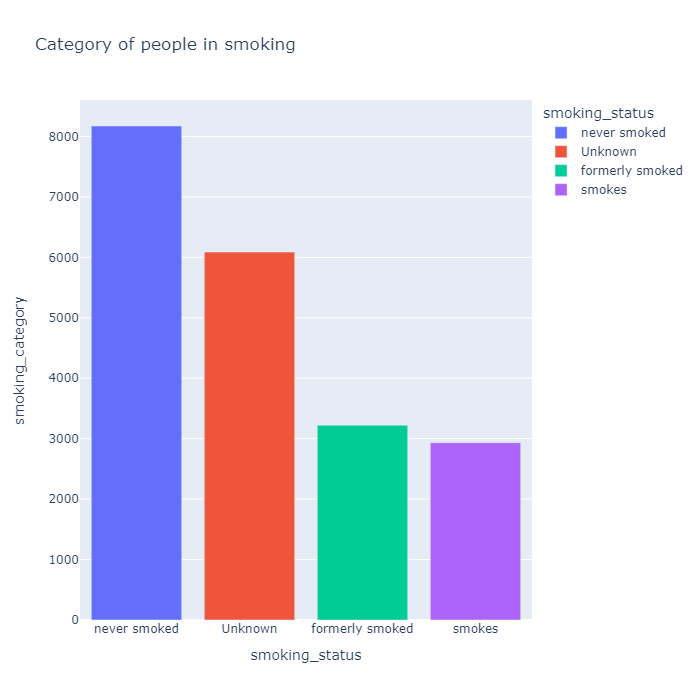
\includegraphics[width=3.589in,height=3.589in]{fig1.png}
\end{center}

\bigskip

{\selectlanguage{english}
\textbf{4.4\ \ References}}

\liststyleWWNumii
\begin{enumerate}
\item {\selectlanguage{english}
Lindsberg, P.J., Roine, R.O. Hyperglycemia in Acute Stroke. Stroke. 2004;35(2):363-364. Available at:
https://doi.org/10.1161/01.STR.0000115297.92132.84. Accessed on: 1 Feb 2004.}
\item {\selectlanguage{english}
L. Liu, {\textquotedbl}Research on Logistic Regression Algorithm of Breast Cancer Diagnose Data by Machine
Learning,{\textquotedbl} 2018 International Conference on Robots \& Intelligent System (ICRIS), Changsha, China, 2018,
pp. 157-160, doi: 10.1109/ICRIS.2018.00049.}
\end{enumerate}
\end{document}
